\section{Task 4: Memory Management on the Stack}

To get the Success! message you have to do a buffer overflow by giving more than 16 characters as input string. After that you can put input chars on the stack. You can set two variables at once, because memory was allocated for variables 'myvalue' and 'mystring'. The stack is first in, last out, i.e. the first element put into it, will be the last one read. Because of this you have to put in the chars in reverse order. The resulting command looks like this:\\

\verb+echo -e "0000000000000000\xef\xbe\xad\xde" | ./memory+


\begin{figure}[ht]
	\centering
	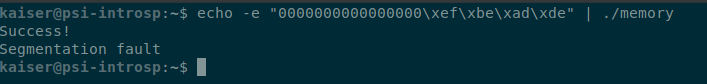
\includegraphics[width=0.8\textwidth]{Assignment0x01/image/success.png}
	\caption{Successful input}
\end{figure}

